\begin{comment}
\subsection{UC29 - Ordinazione piatto}\label{usecase:29}

\begin{figure}[H]
    \centering
    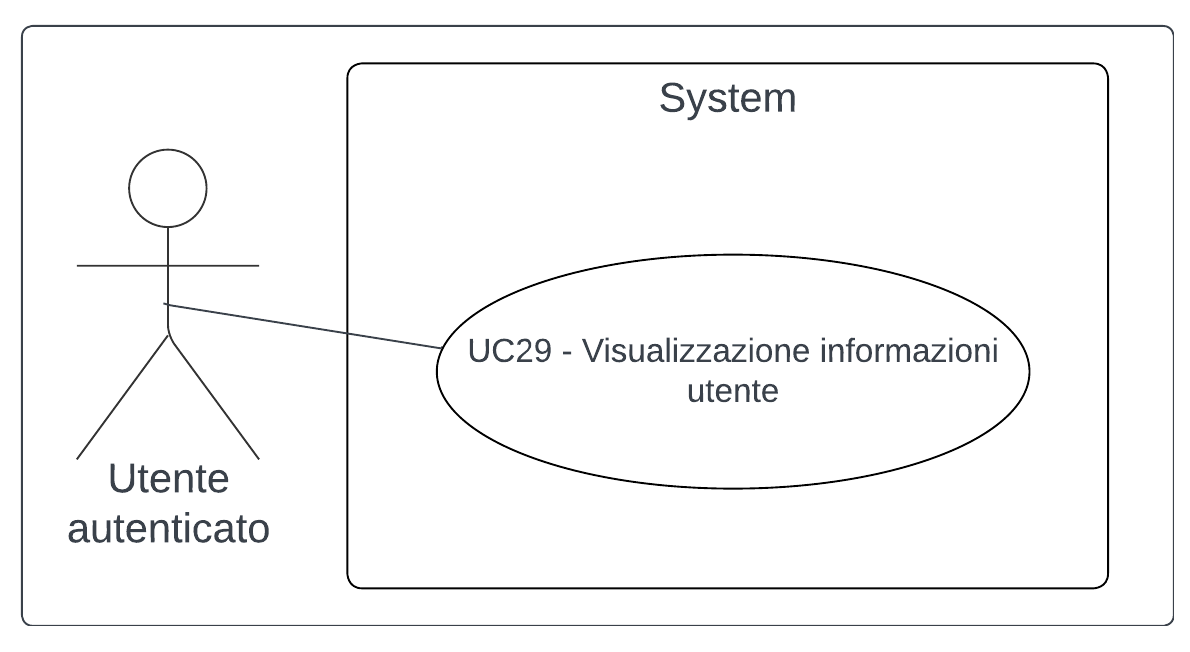
\includegraphics[width=0.9\linewidth]{ucd/UCD29.png}
\end{figure}

\textbf{Attori}:
\begin{itemize}
    \item Utente base autenticato
\end{itemize}
\textbf{Precondizioni}:
\begin{itemize}
    \item L'utente è autenticato dal $\textit{Sistema}_G$ 
    \item L'utente fa parte di una $\textit{Prenotazione}_G$ tavolo valida
    \item Il tempo per l'ordinazione non è scaduto
    \item L'utente ha selezionato un piatto dalla lista dei piatti tramite \nameref{usecase:9}
\end{itemize}
\textbf{Postcondizioni}:
\begin{itemize}
    \item L'utente ha ordinato/modificato il piatto
\end{itemize}
\textbf{Trigger}:
\begin{itemize}
    \item L'utente vuole aggiungere un piatto alla ordinazione collaborativa
\end{itemize}
\textbf{Scenario principale}:
\begin{enumerate}
    \item L'utente visualizza gli ingredienti
    \item L'utente può aggiungere ingredienti
    \item L'utente può rimuovere ingredienti
    \item L'utente conferma il piatto
\end{enumerate}
\newpage
\end{comment}

\subsection{UC29 - Visualizzazione informazioni utente}\label{usecase:29}
\begin{figure}[H]
    \centering
    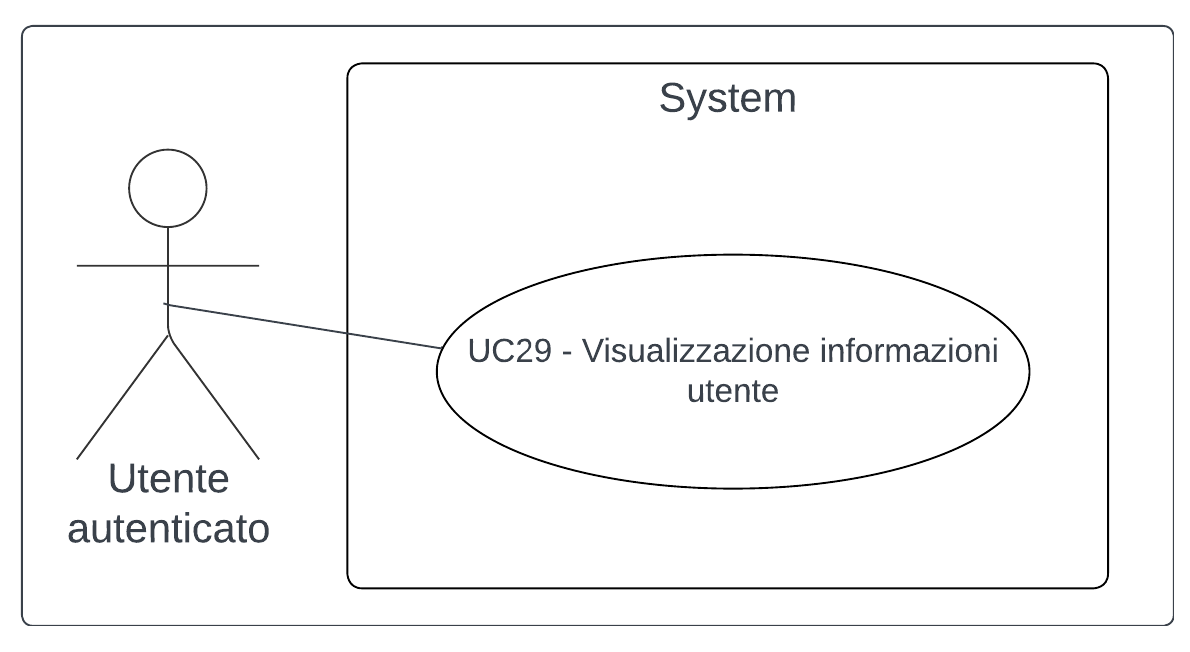
\includegraphics[width=0.9\linewidth]{ucd/UCD29.png}
\end{figure}
\textbf{Attori}:
\begin{itemize}
    \item Utente autenticato
\end{itemize}
\textbf{Precondizioni}:
\begin{itemize}
    \item L'utente ha già creato il suo account
\end{itemize}
\textbf{Postcondizioni}:
\begin{itemize}
    \item L'utente visualizza le informazioni del suo profilo
\end{itemize}
\textbf{Scenario principale}:
\begin{enumerate}
    \item L'utente visualizza le informazioni:
    \begin{enumerate}
        \item Nome
        \item Cognome
        \item Email associata
        \item (Immagine profilo)
        \item Recensioni effettuate
    \end{enumerate}
    \item Se l'utente è amministratore di un ristorante visualizza \nameref{usecase:29_1}
\end{enumerate}